\section{极小极大问题}
\label{sec:minimax-problem}

“先定方案，再承受最坏的响应”，怎样写成一个含义准确的优化问题？

设$\bm{X}\subseteq\mathbb{R}^{n}$，$\bm{Y}\subseteq\mathbb{R}^{q}$是预先给定、互不依赖的非空集合，$f:\bm{X}\times\bm{Y}\to\mathbb{R}$是代价。$\bm{x}$是方案，$\bm{y}$是允许的响应。我们研究
\begin{equation}
 \inf_{\bm{x}\in\bm{X}}\ \sup_{\bm{y}\in\bm{Y}}\ f(\bm{x},\bm{y}),
 \label{eq:minimax-problem}
\end{equation}
称为\term{极小极大问题}（minimax problem）。这个式子要从里往外读：对每个固定的$\bm{x}$，内层求$\bm{x}$所能遭遇的最坏代价；外层在所有方案中选最坏代价最小的那个。

内层面对的是一个已经选定的$\bm{x}$，它不是一个可以脱离外层单独解出来的优化问题。在开头的例子里，$x=0.5$时最坏的$y$是$-1$，$x=-0.5$时最坏的$y$是$1$。单独问“最坏的$y$是什么”没有答案，内层实际上是一族问题，每个$\bm{x}$对应一个。

把内层的$\sup$换成$\inf$，情况完全不同。两层都最小化时，
\[
 \inf_{\bm{x}\in\bm{X}}\inf_{\bm{y}\in\bm{Y}}f(\bm{x},\bm{y})=\inf_{(\bm{x},\bm{y})\in\bm{X}\times\bm{Y}}f(\bm{x},\bm{y}),
\]
两层可以合并成一个联合最小化，这正是第~\ref{chap:block-optimization}章能够交替更新各块的前提。极小极大问题做不到这一点，一个变量要下山，另一个变量要上山，没有一个共同的目标能把两者合起来。

\subsection{响应顺序}
\label{sec:minimax-order}

先用一张有限的代价表看次序的作用。有两个方案$\mathrm{a},\mathrm{b}$和两种扰动，代价如图~\ref{fig:minimax-cost-table}所示。

\begin{BookInlineFigure}
 \centering
 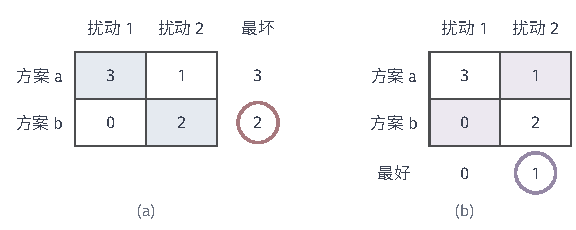
\includegraphics[width=97.5mm]{figures/05-optimization/07-multiple-criteria-and-nested-optimization/tikz/minimax-cost-table/figure.pdf}
 \caption{同一张代价表，两种决策顺序。(a)先定方案：每行取最大（蓝底），最坏列在表右，再在两个最坏值中取小，得到红圈中的$2$。(b)先定扰动：每列取最小（紫底），最好列在表下，再在两个最好值中取大，得到紫圈中的$1$。}
 \label{fig:minimax-cost-table}
\end{BookInlineFigure}

先定方案、再来扰动时，方案$\mathrm{a}$的最坏代价是$3$，方案$\mathrm{b}$的最坏代价是$2$，所以选$\mathrm{b}$，代价是$2$。这就是式~\eqref{eq:minimax-problem}的次序。

反过来，先定扰动、再选方案时，扰动$1$下最好的方案代价是$0$，扰动$2$下最好的方案代价是$1$。扰动一方要让代价大，所以选扰动$2$，代价是$1$。两个次序写成
\[
 \min_{\text{方案}}\max_{\text{扰动}}=2,\qquad\max_{\text{扰动}}\min_{\text{方案}}=1.
\]

同一张表给出两个不同的数。差别来自信息：后选的一方看得到先选的一方，可以对症下药。选方案的一方后选时代价是$1$，先选时代价是$2$，多出来的$1$是先亮底牌的代价。

后选不吃亏这件事不依赖具体的表。

\begin{lemma}[弱极小极大不等式]
\label{lem:minimax-weak}
对任意非空集合$\bm{X},\bm{Y}$和任意$f:\bm{X}\times\bm{Y}\to\mathbb{R}$，
\begin{equation}
 \sup_{\bm{y}\in\bm{Y}}\inf_{\bm{x}\in\bm{X}}f(\bm{x},\bm{y})\leq\inf_{\bm{x}\in\bm{X}}\sup_{\bm{y}\in\bm{Y}}f(\bm{x},\bm{y}).
 \label{eq:minimax-weak}
\end{equation}
\end{lemma}

\begin{proof}
任取$\bm{x}'\in\bm{X}$和$\bm{y}'\in\bm{Y}$。下确界不超过其中任何一项，上确界不小于其中任何一项，所以
\[
 \inf_{\bm{x}\in\bm{X}}f(\bm{x},\bm{y}')\leq f(\bm{x}',\bm{y}')\leq\sup_{\bm{y}\in\bm{Y}}f(\bm{x}',\bm{y}).
\]
最左端不含$\bm{x}'$，最右端不含$\bm{y}'$。左端对$\bm{y}'$取上确界，右端对$\bm{x}'$取下确界，不等号保持。
\end{proof}

连续的例子也一样。回到开头的$f(x,y)=(x-y)^2$，$X=\mathbb{R}$，$Y=[-1,1]$。固定$x$时，$f$是$y$的凸函数，最大值在端点取到，所以
\[
 \sup_{y\in[-1,1]}(x-y)^2=\max\{(x+1)^2,(x-1)^2\}=(\lvert x\rvert+1)^2.
\]

上式在$x=0$处最小，于是先定方案的值是$1$。反过来，无论$y$是多少，后选的$x$都可以取$x=y$，使代价为零，所以先定扰动的值是$0$。图~\ref{fig:minimax-worst-envelope}(a)里，外层最小化的是粗蓝线，而不是任何一条细线。

\begin{BookInlineFigure}
 \centering
 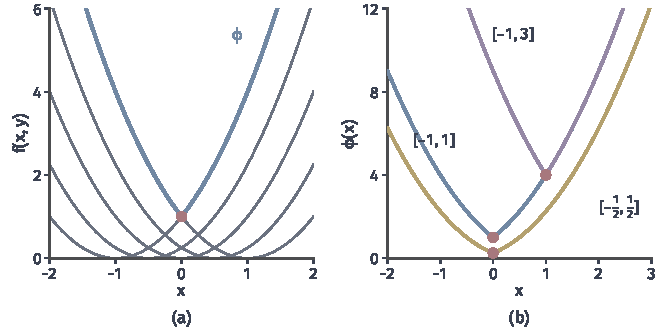
\includegraphics[width=112mm]{figures/05-optimization/07-multiple-criteria-and-nested-optimization/matplotlib/minimax-worst-envelope/figure.pdf}
 \caption{$f(x,y)=(x-y)^2$的最坏代价。(a)灰线是$y=0,\pm\frac12,\pm1$时的$f(\cdot,y)$，蓝线是它们对全部$y\in[-1,1]$的上边缘$\phi(x)=(\lvert x\rvert+1)^2$，红点是外层最优解。(b)三种响应集合下的最坏代价，黄线、蓝线、紫线分别对应标注的集合，红点是各自的最优解。集合$[-1,3]$把最优解移到了$x=1$。}
 \label{fig:minimax-worst-envelope}
\end{BookInlineFigure}

式~\eqref{eq:minimax-weak}的等号一般不成立，上面两个例子都严格小于。所以式~\eqref{eq:minimax-problem}里$\inf$和$\sup$的次序是问题的一部分，不能随手交换。交换需要额外的条件，第~\ref{sec:minimax-saddle}节专门研究。

\subsection{模型边界}
\label{sec:minimax-boundary}

极小极大的结论只对写进模型的$\bm{Y}$负责。“最坏”指的是集合$\bm{Y}$里最坏，集合之外的情形不在保证之内。

图~\ref{fig:minimax-worst-envelope}(b)比较了三个响应集合。对对称的集合$[-\rho,\rho]$，同样的计算给出最坏代价$(\lvert x\rvert+\rho)^2$，最优解都是$x=0$，最优值是$\rho^2$。集合放大时值变大，解却碰巧没动，这很容易让人以为解不依赖集合。

换成不对称的$Y=[-1,3]$，最坏代价变成
\[
 \max\{(x+1)^2,(x-3)^2\}.
\]
两条抛物线在$x=1$相交，最优解是$x=1$，最优值是$4$。按$Y=[-1,1]$选出的$x=0$，放到这个更大的集合下，最坏代价是$(0-3)^2=9$，比$4$差很多。一般地，$\bm{Y}_1\subseteq\bm{Y}_2$时内层上确界只会变大，所以小集合上的最坏值只是大集合上最坏值的下界，小集合上的最优解在大集合上没有任何保证。

\paragraph{Lagrange鞍点是特例}
第~\ref{chap:duality}章已经见过这种结构。约束问题的Lagrange函数$\mathcal{L}$对乘子取上确界时，可行点得到$f(\bm{x})$，不可行点得到$+\infty$，原问题因此写成
\[
 \inf_{\bm{x}\in\bm{D}}\ \sup_{\bm{\lambda}\geq\bm{0},\,\bm{\nu}}\ \mathcal{L}(\bm{x},\bm{\lambda},\bm{\nu}).
\]

这相当于在式~\eqref{eq:minimax-problem}中取$\bm{y}=(\bm{\lambda},\bm{\nu})$，$\bm{Y}=\mathbb{R}^m_{+}\times\mathbb{R}^p$，$\bm{X}=\bm{D}$。对偶问题是交换次序后的$\sup\inf$，弱对偶就是式~\eqref{eq:minimax-weak}。这个特例的结构比一般情形简单，$\mathcal{L}$关于$\bm{y}$是线性的，并且$\bm{Y}$由符号约束给出。本章的$f$不必有这种结构，$\bm{Y}$也可以是任意给定的集合。

\paragraph{本章不讨论的内容}
本章只有一个固定的代价$f$，$\bm{y}$只是“允许的响应”这个数学对象，不代表一个有自身偏好的决策者。模型中各方的偏好、均衡的解释和随时间展开的策略属于另一类问题，可参考\BookChapterRef{chap:static-games-equilibrium}{卷十第8章“静态博弈与均衡”}。这里只研究静态问题~\eqref{eq:minimax-problem}及其数值求解。
